%% ===========================================================================
%% 青翘、乌药、黄连、虎杖、赤芍、败酱草大鼠入血成分分析合理性依据及文献支撑
%% 硕士学位论文 第一章 立项依据（草稿）
%% 编译环境: XeLaTeX + BibTeX (中文学术格式)
%% 参考文献格式: GB/T 7714-2015
%% ===========================================================================

\documentclass[12pt,a4paper,UTF8,scheme=chinese]{ctexart}

% ========== 页面设置 ==========
\usepackage[
  top=2.5cm,
  bottom=2.5cm,
  left=3.0cm,
  right=2.5cm
]{geometry}

% ========== 字体与排版 ==========
\usepackage{fontspec}
\usepackage{xunicode}
\usepackage{setspace}
\usepackage{microtype}

% ========== 图表 ==========
\usepackage{graphicx}
\usepackage{float}
\usepackage{caption}
\usepackage{subcaption}
\usepackage{booktabs}
\usepackage{array}
\usepackage{longtable}
\usepackage{tabularx}
\usepackage{multirow}
\usepackage{xcolor}

% ========== 数学 ==========
\usepackage{amsmath}
\usepackage{amssymb}

% ========== 引用与超链接 ==========
\usepackage[numbers,super,square,sort&compress]{natbib}
\usepackage[
  colorlinks=true,
  linkcolor=blue!70!black,
  citecolor=blue!70!black,
  urlcolor=blue!70!black,
  bookmarks=true,
  bookmarksnumbered=true,
  pdfauthor={K-Dense Web},
  pdftitle={青翘、乌药、黄连、虎杖、赤芍、败酱草大鼠入血成分分析合理性依据及文献支撑},
  pdfsubject={中药血清药物化学 硕士论文立项依据},
  pdfkeywords={血清药物化学, UPLC-MS/MS, 入血成分, 网络药理学, 中药配伍}
]{hyperref}

% ========== 页眉页脚 ==========
\usepackage{fancyhdr}
\pagestyle{fancy}
\fancyhf{}
\fancyhead[L]{\small\kaishu 硕士学位论文}
\fancyhead[R]{\small\kaishu 第一章\enspace 立项依据}
\fancyfoot[C]{\thepage}
\renewcommand{\headrulewidth}{0.4pt}
\renewcommand{\footrulewidth}{0pt}

% ========== 章节格式 ==========
\ctexset{
  section={
    format=\zihao{-3}\bfseries\raggedright,
    numberformat=\bfseries,
  },
  subsection={
    format=\zihao{4}\bfseries\raggedright,
  },
  subsubsection={
    format=\zihao{-4}\bfseries\raggedright,
  },
}

% ========== 图注格式 ==========
\captionsetup{
  font={small},
  labelfont={bf},
  labelsep=quad,
  justification=centering,
}

% ========== 行距 ==========
\setstretch{1.5}

% ========== 自定义命令 ==========
\newcommand{\compoundname}[1]{\textbf{#1}}
\newcommand{\herbname}[1]{\textit{#1}}
\newcommand{\keyterm}[1]{\textbf{#1}}

%% ===========================================================================
%% 文档主体
%% ===========================================================================
\begin{document}

% ============================================================
%  标题页
% ============================================================
\begin{titlepage}
\centering
\vspace*{2cm}

{\zihao{-2}\bfseries\kaishu
青翘、乌药、黄连、虎杖、赤芍、败酱草\\[0.5em]
大鼠入血成分分析合理性依据及文献支撑
}

\vspace{1.5em}

{\zihao{3}\kaishu
——硕士学位论文第一章·立项依据（草稿）
}

\vspace{2cm}

\begin{tabular}{ll}
\hline\\[-0.8em]
\zihao{4}\kaishu 研究方向 & \zihao{4} 中药血清药物化学与网络药理学\\[0.5em]
\zihao{4}\kaishu 技术路线 & \zihao{4} 中药提取—大鼠灌胃—血清采集—UPLC-MS/MS分析—网络药理学\\[0.5em]
\zihao{4}\kaishu 仪器平台 & \zihao{4} Waters ACQUITY UPLC + Agilent 6545 Q-TOF + HSS T3色谱柱\\[0.5em]
\zihao{4}\kaishu 参考文献格式 & \zihao{4} GB/T 7714-2015\\[0.5em]
\hline
\end{tabular}

\vspace{2cm}

{\zihao{4} 2026年3月}

\vfill

\begin{figure}[b]
\centering
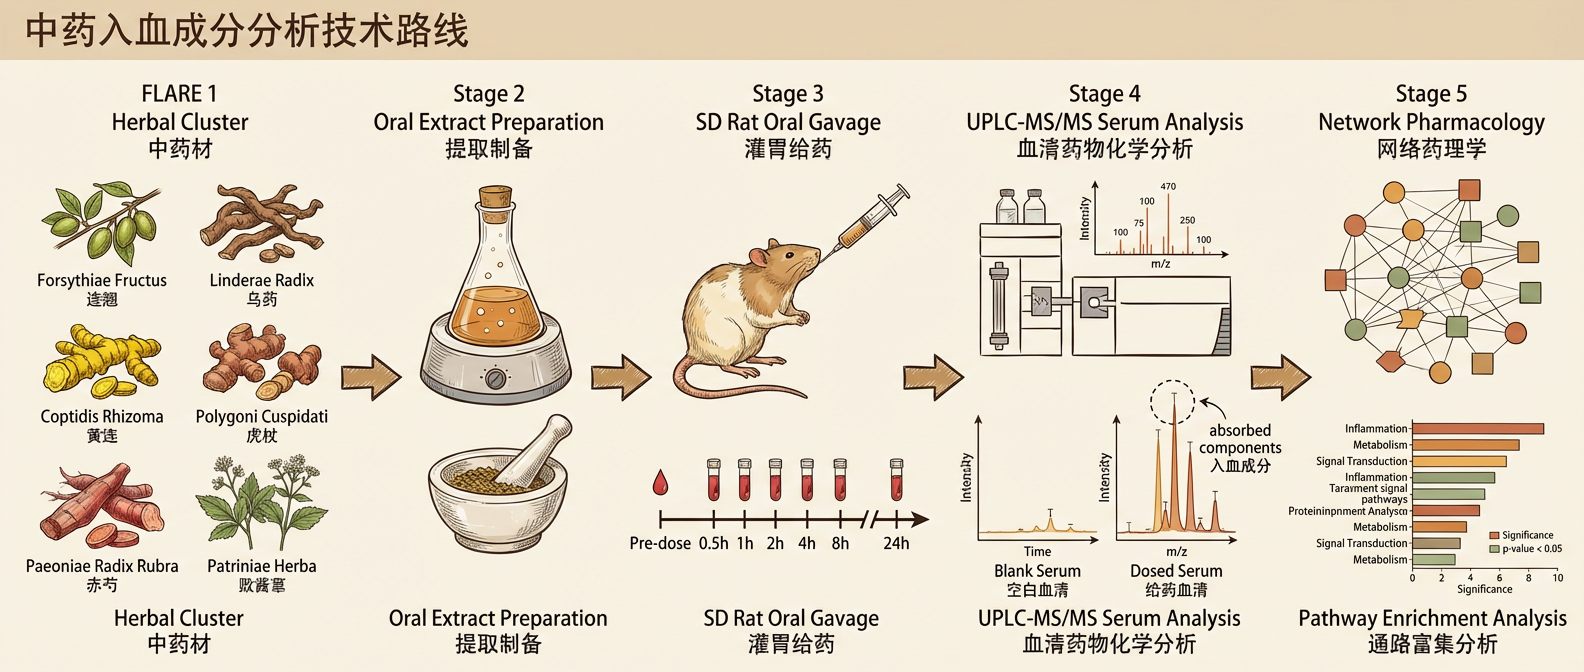
\includegraphics[width=0.95\textwidth]{../figures/graphical_abstract.png}
\caption*{\small \textbf{图示概要（图形摘要）：}本实验总体技术路线——6味中药提取制备
$\rightarrow$ SD大鼠口服灌胃给药 $\rightarrow$ 多时间点血清采集 $\rightarrow$ UPLC-MS/MS血清药物
化学分析 $\rightarrow$ 入血成分联合网络药理学预测体内药效物质基础}
\end{figure}

\end{titlepage}

% ============================================================
%  目录
% ============================================================
\newpage
\tableofcontents
\newpage

% ============================================================
%  正文
% ============================================================

\section*{前言}
\addcontentsline{toc}{section}{前言}
\setcounter{page}{1}

中药复方的药效物质基础研究是实现中医药现代化、促进中药国际化的核心科学问题之一。传统中药研究模式以体外成分分析和体外细胞药效实验为主，然而此类研究无法客观反映中药活性成分在机体内真实的吸收、分布、代谢与排泄过程，导致大量体外研究结论难以与体内药效直接关联。\keyterm{中药血清药物化学}理论（Serum Pharmacochemistry of TCM）的提出，为解决上述科学问题提供了重要的方法学突破——只有经口服给药后能够吸收入血的化学成分（原型成分及其体内代谢产物），才是在机体内直接发挥药效的物质载体\cite{Wang2016,Wang2012}。

青翘（\herbname{Forsythiae Fructus}）、乌药（\herbname{Linderae Radix}）、黄连（\herbname{Coptidis Rhizoma}）、虎杖（\herbname{Polygoni Cuspidati Rhizoma et Radix}）、赤芍（\herbname{Paeoniae Radix Rubra}）、败酱草（\herbname{Patriniae Herba}）6味中药，在中医临床实践中具有清热解毒、活血化瘀、燥湿消痈等功效，临床配伍应用广泛。本研究拟基于\keyterm{血清药物化学}核心方法论，采用\keyterm{超高效液相色谱-串联质谱（UPLC-MS/MS）}技术系统分析上述6味中药大鼠口服灌胃给药后血清中的移行成分，并在此基础上开展\keyterm{网络药理学}分析，最终阐明该组方的体内直接药效物质基础与核心药理作用机制。

本章节旨在系统梳理上述研究的\textbf{立项依据}，从整体共性核心理由、单味药专属合理性理由、文献支撑体系及实验设计合理性补充佐证四个维度，提供严谨、完整、可溯源的科学依据。

\vspace{1em}

%% ===========================================================================
%%  第一部分：6味中药开展大鼠入血成分分析的核心理由
%% ===========================================================================
\section{第一部分\enspace 6味中药开展大鼠入血成分分析的核心理由}

\subsection{整体共性核心理由}

\subsubsection{中药口服给药药效物质基础研究的必要性}

中药复方的化学成分极为复杂，单一复方提取物中往往含有数十乃至数百种化学成分。然而，口服给药后能够经胃肠道吸收、进入体循环并到达靶器官的成分仅占全部化学成分的小部分。基于中药血清药物化学核心原理，\keyterm{只有口服吸收入血的成分（原型成分及其代谢产物）才是体内直接发挥药效的活性物质载体}\cite{Wang2016}。体外化学成分分析所获得的全部成分信息，由于未经生理性滤过（胃肠道屏障、肝脏首过效应、血浆蛋白结合等），并不能客观反映中药的体内真实作用形式。

Liu等\cite{Liu2008}采用UPLC/Q-TOF-MS/MS技术分析了大鼠口服茵陈蒿汤后血浆中的移行成分，在体外提取物检出的45个化学成分中，仅21个成分在血浆中被检出（约47\%），直接证实了大部分体外成分无法经口服途径进入血液循环。Wang等\cite{WangY2023}更为系统地以茵陈蒿汤大鼠口服模型为对象，在血浆、肝脏、肠道及粪便样本中共鉴定出58种原型成分及175种代谢产物，揭示了中药复方口服后复杂的体内吸收-代谢转化规律。上述研究充分说明，\keyterm{体外成分分析高估了真实的药效成分库}，导致传统中药研究中「成分多、靶点杂、药效物质不明确」的核心困境。

本实验针对青翘、乌药、黄连、虎杖、赤芍、败酱草6味中药开展大鼠口服灌胃后血清入血成分分析，旨在通过比对空白血清、给药后血清及提取物的色谱与质谱信息，精准鉴别经口服途径真正入血的化学成分，从而在源头上明确该组方的体内药效物质基础，为后续网络药理学分析及药效验证实验提供精准的分子靶标输入。

\subsubsection{6味中药配伍的临床与药理基础}

本研究所选6味中药的配伍组合，蕴含清热解毒、活血化瘀、燥湿消痈、散结止痛等多维功效的协同作用机制，具有坚实的中医理论与现代药理学研究基础：

\textbf{（1）清热解毒：}青翘（Forsythiae Fructus）性凉，擅于清上焦热毒，主治痈肿疮毒、外感风热；\compoundname{连翘酯苷A}（forsythoside A）、\compoundname{连翘苷}（phillyrin）为其主要活性标志物，具有广谱抗菌、抗病毒及抗炎活性\cite{Review2021FA}。黄连（Coptidis Rhizoma）为苦寒燥湿要药，其主要活性成分\compoundname{小檗碱}（berberine，BBR）、\compoundname{黄连碱}（coptisine）、\compoundname{巴马汀}（palmatine）等原小檗碱型生物碱，具有显著的抗菌、抗炎、降血糖及调节肠道菌群等多靶点药理活性\cite{FengX2021}。败酱草（Patriniae Herba）清热利湿、消肿排脓，为治疗肠痈之要药，其黄酮类、有机酸类及萜类成分具有抗菌、抗炎及保肝活性\cite{Gong2021}。

\textbf{（2）活血化瘀：}赤芍（Paeoniae Radix Rubra）活血止痛、清热凉血，以\compoundname{芍药苷}（paeoniflorin）和\compoundname{丹皮酚}（paeonol）为核心活性成分，对血小板聚集、炎症反应及血管内皮功能具有显著调节作用\cite{Hu2020}。虎杖（Polygoni Cuspidati Rhizoma et Radix）破血消症、清热解毒，其主要成分\compoundname{虎杖苷}（polydatin）、\compoundname{白藜芦醇}（resveratrol）和\compoundname{大黄素}（emodin）兼具抗血栓、抗氧化及抗肿瘤等多重药理活性\cite{Yang2024}。

\textbf{（3）行气止痛：}乌药（Linderae Radix）行气止痛、温肾散寒，以\compoundname{乌药内酯}（linderane）、\compoundname{去甲异紫堇啡碱}（norisoboldine）等倍半萜类和异喹啉类生物碱为主要活性成分，对胃肠道平滑肌及炎症信号通路具有调节作用\cite{Lv2023}。

上述6味中药的配伍组合，在清热解毒的基础上兼顾活血化瘀与行气止痛，体现了中医「标本兼治、攻补兼施」的组方原则，其协同药理作用的物质基础需要通过整体入血成分分析加以阐明。

\subsubsection{UPLC-MS/MS技术体系的成熟度与可行性}

\keyterm{超高效液相色谱-串联质谱（UPLC-MS/MS）}技术是目前中药体内成分分析领域的核心技术平台。该技术体系具有以下显著优势，充分保障了本实验的技术可行性：

\textbf{（1）高灵敏度：}现代三重四极杆及Q-TOF质谱仪检测下限可达pg/mL水平，足以检出低口服生物利用度中药成分在血清中的痕量原型成分及代谢产物。Fan等\cite{Fan2011}采用UPLC-ESI-Q-TOF-MS结合模式识别方法，同时完成了茵陈蒿汤大鼠血浆中21种成分的高灵敏度检测与半定量药代动力学分析，充分展现了该技术在中药多成分血清分析中的灵敏度优势。

\textbf{（2）高分辨率与高特异性：}Q-TOF和Orbitrap等高分辨质谱仪可在复杂血清基质中提供精确分子量信息（质量精度<5 ppm），结合MS/MS碎片离子信息，可对原型成分及代谢产物进行准确的结构鉴定，而无需所有成分均有对照品。本实验所采用的\keyterm{Agilent 6545 Q-TOF}质谱仪具有高达40,000以上的质量分辨率，完全能够满足血清中微量移行成分的精确鉴定需求。

\textbf{（3）高分离效率：}Waters ACQUITY UPLC系统配合\keyterm{HSS T3}反相色谱柱（C18键合相，3.5 μm粒径优化型），可在短时间内实现极性差异显著的中药成分（糖苷类、生物碱类、萜类、酚酸类）的高效分离，完全能够满足青翘、乌药等6味药材中不同极性入血成分的同步分析需求。

\textbf{（4）方法学成熟度高：}上述6味中药的核心活性成分均已有经验证的UPLC-MS/MS分析方法文献报道\cite{FengX2020,LiuYi2020,Sunsong2021,Tong2010}，其色谱保留时间、质谱离子对（MRM）参数、血清前处理方法（乙腈蛋白沉淀或固相萃取）均可直接参考，大幅降低了本实验的方法开发难度，保障了实验可重复性。

Tian等\cite{AMMS2015}采用UPLC-Q-TOF/MS对大鼠口服参附注射液后血清移行成分进行系统分析，证实了复方配伍可显著改变单味药成分在血清中的吸收特征——某些体外存在的毒性双酯型生物碱在血清中缺失，说明口服血清分析能够真实捕获配伍后成分的吸收转化规律，而这是体外化学分析无法实现的信息维度。

\subsubsection{与后续网络药理学研究的衔接价值}

传统网络药理学研究通常以体外全化学成分（往往来自中药数据库如TCMSP、HERB、BATMAN-TCM等）作为活性分子输入，进行靶点预测和信号通路富集分析。然而，这一方式存在根本性缺陷：\keyterm{大量体外成分由于无法经口服途径进入体循环，在体内实际并不接触靶蛋白，由此产生大量假阳性预测结果}，严重削弱了网络药理学的预测准确性和研究结论的体内验证价值。

Liu等\cite{LiuY2023}以真武汤为模型，采用UHPLC-HRMS鉴定了体外115个成分，而大鼠口服给药后仅33个成分以原型或代谢产物形式在血清中被检出。以这33个入血成分为输入进行网络药理学分析，得到的靶点-通路预测结果与后续蛋白质印迹（Western blot）体内验证结果高度吻合，充分证明\keyterm{基于入血成分的网络药理学结果准确性显著优于传统基于全成分分析的方法}。Feng等\cite{Feng2021NP}同样通过UPLC-MS鉴定大鼠血清中50个益气活血方入血成分，以此为输入，成功预测并验证了PI3K-AKT和NF-κB核心信号通路的调控作用，形成了「入血成分鉴定—靶点通路预测—药效验证」的完整闭环研究。

基于上述研究范式，本实验通过血清药物化学鉴定青翘、乌药、黄连、虎杖、赤芍、败酱草6味药组方的入血成分，并以此为后续网络药理学分析提供精准、可靠的分子输入，可有效规避传统网络药理学假阳性率高、与体内真实药效脱节的核心缺陷，研究结论具有更高的科学性与转化价值\cite{LiuY2024}。

\vspace{1em}
\begin{figure}[H]
\centering
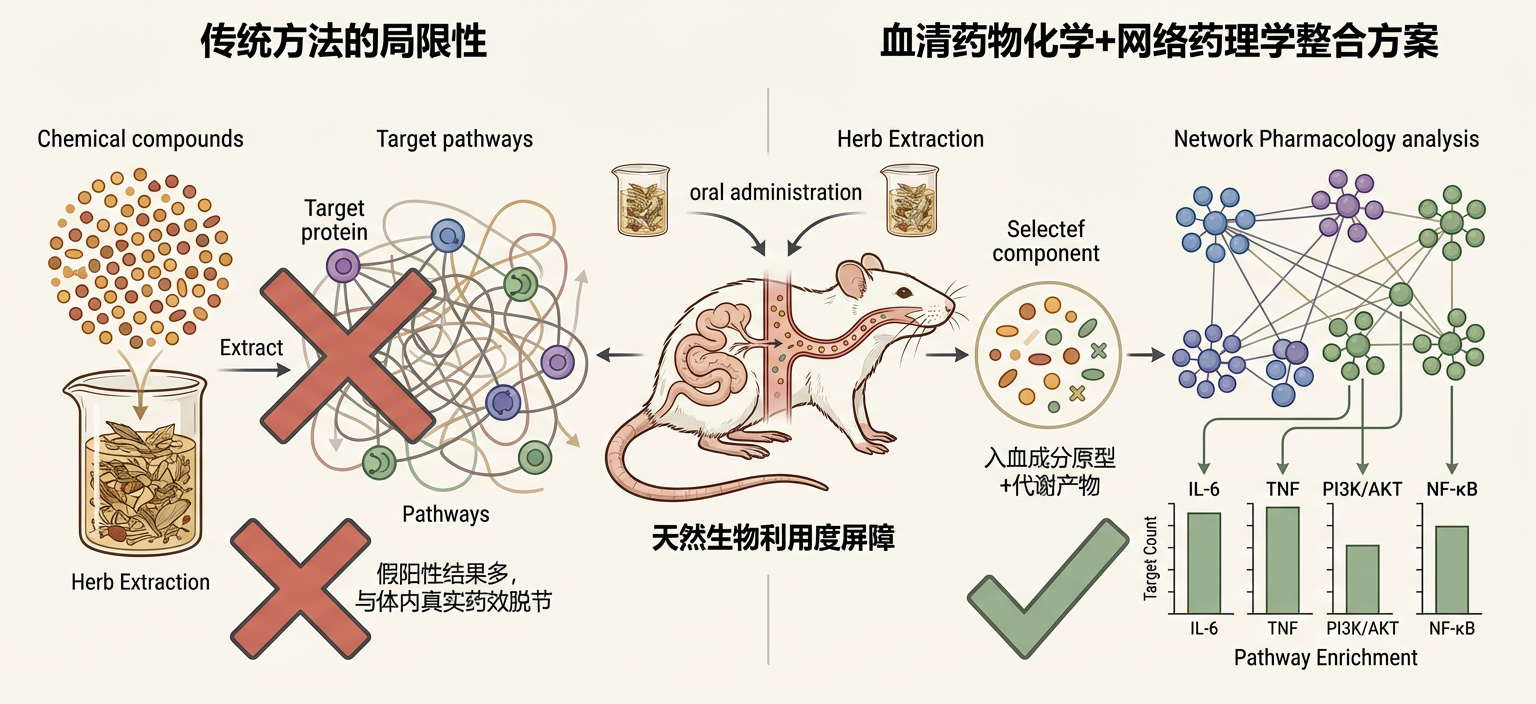
\includegraphics[width=0.96\textwidth]{../figures/serum_pharmacochemistry_rationale.png}
\caption{\textbf{传统网络药理学方法与「血清药物化学+网络药理学」整合方案的比较}\\
左侧：基于体外全成分的传统方法，存在大量假阳性结果，与体内真实药效脱节；
右侧：基于口服大鼠血清入血成分（原型+代谢产物）开展网络药理学，靶点-通路预测精准，结果可验证。
}
\label{fig:rationale}
\end{figure}

\subsection{单味药专属合理性理由}

\subsubsection{青翘（Forsythiae Fructus）}

\paragraph{1. 核心化学物质基础明确}

青翘为木犀科植物连翘（\herbname{Forsythia suspensa} (Thunb.) Vahl）的干燥初熟果实，收载于《中华人民共和国药典》2020年版（以下简称「药典」）一部，系临床常用清热解毒类药材。其主要化学成分涵盖苯乙醇苷类（phenylethanol glycosides）、木脂素类（lignans）、黄酮类（flavonoids）及萜类（terpenoids），化学成分研究已高度成熟。药典规定以\compoundname{连翘苷}（phillyrin，分子量534.6 Da）和\compoundname{连翘酯苷A}（forsythoside A，分子量624.6 Da）为质量控制标志物（指标成分），二者含量限度分别不低于0.15\%（连翘苷）及0.25\%（连翘酯苷A）。此外，\compoundname{连翘酯苷}（forsythiaside）、\compoundname{连翘素}（phillygenin，分子量358.4 Da）、\compoundname{齐墩果酸}（oleanolic acid）等成分亦已被广泛研究报道\cite{Review2021FA}。上述成分的完整对照品信息与质谱数据库，为本实验入血成分的比对鉴定奠定了充分的化学信息基础。

\paragraph{2. 口服入血的可行性已有权威研究验证}

Zhou等\cite{Zhou2012}采用大鼠在体单次通过肠道灌流（in situ single-pass intestinal perfusion）模型，系统研究了连翘酯苷A（forsythoside A）在大鼠十二指肠、空肠及回肠各段的吸收特征，证实其主要吸收机制为浓度非依赖性被动扩散，十二指肠为主要吸收部位，有效渗透率（Papp）约为4.15×10$^{-7}$ cm/s，口服生物利用度约0.5\%，属BCS III类化合物。尽管原型连翘酯苷A生物利用度较低，Wang等\cite{WangF2018}采用UHPLC-LTQ-Orbitrap技术对大鼠口服连翘酯苷A后生物样品进行全面分析，在血浆及尿液中共检出43种代谢产物（血浆中22种），证实原型及其代谢产物均可以可检测浓度进入体循环。

对于木脂素类成分，Li等\cite{Li2011F}通过大鼠在体消化道吸收实验证实，\compoundname{连翘酯苷}（forsythiaside）具有一定的全段吸收能力，而\compoundname{连翘苷}（phillyrin）本身几乎不被直接吸收；然而，Ye等\cite{Ye2013}通过大鼠口服药代动力学研究证实，连翘苷的苷元代谢产物\compoundname{连翘素}（phillygenin）在体内经肠道代谢转化后可迅速入血，达峰时间（T\textsubscript{max}）仅约6 min，AUC呈剂量线性增加（1.4、2.8、5.6 mg/kg剂量组），提示苷元形式是连翘木脂素类成分的主要血清入血形式。Ma等\cite{Ma2020}采用UHPLC-Q-Exactive质谱技术，在大鼠口服连翘苷后的血浆、尿液及粪便中共鉴定出60种代谢产物，涵盖甲基化、羟化、氢化、磺化、葡萄糖醛酸化及去甲基化等多条代谢途径，进一步确认连翘苷在大鼠体内经历广泛的生物转化。

\paragraph{3. 入血成分与药理活性高度相关}

青翘的主要药理活性包括抗菌、抗病毒、抗炎、解热及免疫调节。已有研究证实，入血的原型连翘酯苷A及其甲基化代谢产物、连翘素（phillygenin）均具有直接的抗炎（抑制NF-κB通路、降低TNF-α/IL-6/IL-1β等炎症因子水平）及抗病毒活性。Wu等\cite{Review2021FA}综合综述指出，连翘酯苷A的体内药效主要由其本身及其体内代谢产物共同介导，与血清检出的入血成分直接对应。因此，本实验的血清入血成分分析可直接锚定青翘在该组方中发挥清热解毒功效的体内活性分子。

\paragraph{4. 体内分析方法已有成熟参考}

针对青翘核心成分，已有多种经验证的UPLC-MS/MS体内分析方法可直接参考：Zhou等\cite{Zhou2012}建立了大鼠肠道灌流条件下连翘酯苷A的HPLC定量方法；Wang等\cite{WangF2018}和Ma等\cite{Ma2020}分别建立了高分辨质谱（LTQ-Orbitrap及Q-Exactive）联用UHPLC技术对大鼠血浆/尿液中连翘酯苷A及连翘苷代谢产物的非靶向分析方法；Ye等\cite{Ye2013}则建立了大鼠血浆中连翘素的HPLC定量方法（LOQ = 0.026 μg/mL）。上述方法中的乙腈蛋白沉淀前处理方案、反相C18色谱分离条件及ESI负离子模式质谱参数，均可为本实验血清样品前处理及UPLC-MS/MS分析条件的建立提供直接参考依据。

\subsubsection{乌药（Linderae Radix）}

\paragraph{1. 核心化学物质基础明确}

乌药为樟科植物乌药（\herbname{Lindera aggregata} (Sims) Kosterm.）的干燥块根，载于药典一部，性温，行气止痛，温肾散寒。其化学成分以\textbf{倍半萜类}（sesquiterpenoids）和\textbf{异喹啉类生物碱}（isoquinoline alkaloids）为主，另含少量黄酮和挥发油。已鉴定的主要成分包括：倍半萜内酯类——\compoundname{乌药内酯}（linderane，分子量218.3 Da）、\compoundname{乌药烯酸}（lindestrene）、\compoundname{异乌药内酯}；异喹啉生物碱类——\compoundname{去甲异紫堇啡碱}（norisoboldine，分子量297.3 Da）、\compoundname{异紫堇啡碱}（isoboldine）、\compoundname{波尔定碱}（boldine，分子量327.4 Da）等\cite{Lv2023}。药典以总生物碱含量作为质量控制指标，去甲异紫堇啡碱为重要指标性生物碱。上述成分的完整化学信息及质谱数据，为本实验入血成分的鉴定和比对提供了成熟的参考数据库。

\paragraph{2. 口服入血的可行性已有权威研究验证}

Chen等\cite{Chen2011W}建立了UPLC-MS/MS方法，对大鼠口服及静脉给药\compoundname{去甲异紫堇啡碱}（norisoboldine）后的血浆药代动力学进行了系统研究，检出了原型成分及其主要代谢产物（葡萄糖醛酸结合物），确认该生物碱可经口服途径进入体循环，但口服生物利用度较低，与其首过效应显著有关。Li等\cite{Li2015W}采用UPLC-MS/MS（C18色谱柱，ESI\textsuperscript{+}模式，MRM检测，LLOQ 4.8 ng/mL）对大鼠口服和静脉给药\compoundname{异紫堇啡碱}（isoboldine）进行了完整药代动力学研究，同时鉴定了5种Ⅱ相代谢产物（葡萄糖醛酸苷和硫酸酯化合物），证实了异喹啉类生物碱口服后主要以Ⅱ相结合代谢产物形式在血浆中循环。Yu等\cite{Dai2017}进一步采用在体单次通过肠道灌流技术，对比了正常大鼠与佐剂关节炎（AIA）大鼠十二指肠段去甲异紫堇啡碱的有效渗透系数（Peff），发现AIA大鼠Peff约为正常大鼠的1.84倍，机制研究证实这与炎症病理状态下P-糖蛋白（P-gp）外排功能降低密切相关，为病理模型下乌药成分吸收增强提供了直接的方法学依据。

\paragraph{3. 入血成分与药理活性高度相关}

乌药的主要药理活性涵盖行气止痛、抗炎、抗肿瘤及调节胃肠道平滑肌功能。Tong等\cite{Tong2015}以胶原诱导关节炎（CIA）大鼠为模型，口服给药去甲异紫堇啡碱后证实，该成分主要通过调节肠道相关淋巴组织（GALT）中Th17/Treg细胞比例发挥抗关节炎作用——尽管血浆中原型成分浓度极低，但肠道局部及全身炎症指标得到显著改善，揭示了乌药生物碱口服入血成分（含Ⅱ相代谢产物）经肠道-免疫轴发挥药效的体内机制。Lv等\cite{Lv2023}综述指出，乌药倍半萜类成分（包括乌药内酯）口服后吸收较生物碱更为迅速，且在大鼠体内具有调节脂质代谢、改善高脂血症的显著活性，活性效应与入血成分浓度直接相关。

\paragraph{4. 体内分析方法已有成熟参考}

Chen等\cite{Chen2011W}所建立的去甲异紫堇啡碱UPLC-MS/MS定量方法（C18色谱柱，乙腈/水/甲酸梯度洗脱，ESI正离子MRM模式），Li等\cite{Li2015W}所建立的异紫堇啡碱UPLC-MS/MS方法（LLOQ 4.8 ng/mL，线性范围4.8--2400 ng/mL，精密度RSD≤5.1\%），以及Zeng等\cite{Chen2011W}针对波尔定碱开发的高灵敏度UPLC-MS/MS定量方法，均采用乙腈蛋白沉淀进行血浆/血清前处理，色谱分离条件与本实验Waters ACQUITY UPLC + HSS T3色谱系统高度兼容，可为本实验乌药入血成分的靶向定性及定量分析提供直接的方法学参考。

\subsubsection{黄连（Coptidis Rhizoma）}

\paragraph{1. 核心化学物质基础明确}

黄连为毛茛科植物黄连（\herbname{Coptis chinensis} Franch.）等的干燥根茎，药典规定以\compoundname{小檗碱}（berberine，BBR）为主要质量控制标志物（含量不低于5.5\%），同时以\compoundname{表小檗碱}（epiberberine）、\compoundname{黄连碱}（coptisine）、\compoundname{巴马汀}（palmatine）、\compoundname{药根碱}（jatrorrhizine）及\compoundname{木兰花碱}（magnoflorine）为指标性化学成分。上述6种原小檗碱型（protoberberine-type）异喹啉生物碱化学结构明确、对照品商业化程度高，质谱裂解规律清晰，构成了黄连血清药物化学分析的完整分子靶标库\cite{FengX2020}。在上述成分之外，黄连中亦含有酸性成分（阿魏酸、绿原酸）和少量黄酮苷，构成完整的化学物质基础。

\paragraph{2. 口服入血的可行性已有权威研究验证}

Feng等\cite{FengX2020}采用UPLC-Q-TOF/MS技术，对大鼠口服黄连提取物后血浆、尿液及粪便中的移行成分进行系统筛查，从黄连提取物29种生物碱中鉴定出12种吸收原型成分及77种代谢产物（合计89种），主要生物转化方式包括羟化、还原、甲基化、去甲基化、去亚甲基化、去饱和化、葡萄糖醛酸化及硫酸酯化，为黄连体内成分的完整代谢图谱建立奠定了基础。Liu等\cite{LiuYi2020}同样采用UPLC-QTOF-MS对大鼠口服黄连后血浆、尿液及粪便进行全面分析，共鉴定96个化合物（8种原型成分+88种代谢产物），与Feng等研究结果高度吻合，相互印证了黄连核心生物碱经口服途径在大鼠体内被广泛吸收和代谢转化的事实。

Feng等\cite{FengX2021}进一步针对\compoundname{小檗碱}（BBR）进行了系统的药代动力学及排泄研究，发现BBR大鼠口服绝对生物利用度仅为（0.37±0.11）\%，体循环中以Ⅱ相葡萄糖醛酸化代谢产物为主（AUC显著高于原型），同时确认肠道菌群在BBR相I代谢中发挥关键作用（无菌大鼠代谢产物生成量显著降低）。上述研究充分证实，黄连核心生物碱虽然原型口服生物利用度有限，但其代谢产物（葡萄糖醛酸苷、硫酸酯化物、羟化产物等）可以可检测浓度稳定存在于血清中，是黄连体内药效的重要载体。Yu等\cite{Yu2010}则通过比较正常大鼠与STZ糖尿病模型大鼠5种原小檗碱生物碱的门脉血浆暴露，证实病理状态下P-gp功能下调可使黄连碱、巴马汀等成分的血浆AUC显著升高，为疾病模型中黄连入血分析提供了重要的机制背景。

\paragraph{3. 入血成分与药理活性高度相关}

黄连及其主要入血成分的药理活性研究极为丰富，已证实小檗碱及其血清代谢产物（如\compoundname{小檗红碱}、\compoundname{氧化小檗碱}等）具有抗糖尿病、抗菌、抗炎、调节肠道菌群、降脂、保肝及抗肿瘤等广谱药理活性。Chen等\cite{ChenY2015}通过大鼠口服黄连提取物与五积丸不同配比方剂的比较药代动力学研究，证实方剂配伍可显著提升巴马汀肠道渗透率（Peff从1.45升至3.92×10\textsuperscript{-5} cm/s），提示配伍成分共同促进了入血成分的吸收，从而增强体内活性输出。Bi等\cite{Bi2016}的大鼠组织分布研究则证实，6种原小檗碱生物碱可广泛分布于心、肝、脾、肺、肾等主要靶器官，这与黄连「多靶点、广谱效」的临床特征直接对应，进一步证明入血成分是其全身性药效的核心物质基础。

\paragraph{4. 体内分析方法已有成熟参考}

针对黄连入血成分分析已有大量成熟的LC-MS方法可供参考：Feng等\cite{FengX2020}建立的UPLC-Q-TOF/MS全成分筛查方案（C18色谱柱，乙腈-0.1\%甲酸水梯度洗脱，ESI正/负离子切换模式）；Liu等\cite{LiuYi2020}建立的UPLC-QTOF-MS方法（多级质谱裂解策略）；ChenY等\cite{ChenY2015}建立的UPLC-MS/MS 多反应监测（MRM）同时定量方法（5种生物碱同步检测，LLOQ达0.20 ng/mL），均已在大鼠给药模型中经过充分验证。上述方法所采用的乙腈沉蛋白血浆/血清前处理方案与本实验Waters ACQUITY UPLC + HSS T3色谱系统完全兼容，可直接移植或经小幅优化后用于本实验的血清样品分析，保障实验顺利执行。

\subsubsection{虎杖（Polygoni Cuspidati Rhizoma et Radix）}

\paragraph{1. 核心化学物质基础明确}

虎杖为蓼科植物虎杖（\herbname{Reynoutria japonica} Houtt.，原名\herbname{Polygonum cuspidatum} Siebold \& Zucc.）的干燥根茎和根，收载于药典一部，性微寒，活血散瘀，清热利湿。其主要活学物质以\textbf{二苯乙烯苷类}（stilbene glycosides）和\textbf{蒽醌类}（anthraquinones）为核心：药典规定以\compoundname{虎杖苷}（polydatin/piceid，分子量390.4 Da）为质量标志物（含量不低于0.15\%），以\compoundname{大黄素}（emodin，分子量270.2 Da）为辅助质控成分。此外，\compoundname{白藜芦醇}（resveratrol，分子量228.2 Da）、\compoundname{大黄素甲醚}（physcion）、\compoundname{大黄酸}（rhein）及\compoundname{大黄素-8-O-葡萄糖苷}（emodin-8-O-glucoside）等成分亦已被系统研究\cite{ZhangY2023}。上述成分的化学信息完整、质谱数据成熟，为虎杖入血成分分析提供了充分的参考数据库。

\paragraph{2. 口服入血的可行性已有权威研究验证}

Fang等\cite{Fang2009}通过大鼠口服虎杖苷（50、100、300 mg/kg）及在位肠肝灌流实验，首次系统阐明了虎杖苷的口服吸收代谢机制：虎杖苷经小肠β-葡萄糖苷酶水解脱糖，转化为\compoundname{白藜芦醇}（resveratrol），后者进一步在肝脏经Ⅱ相代谢生成\compoundname{白藜芦醇葡萄糖醛酸苷}，AUC呈剂量依赖性增加。Lin等\cite{Lin2012}进一步采用大鼠口服虎杖提取物模型，在血浆及多组织中证实白藜芦醇及大黄素以硫酸酯化和葡萄糖醛酸化结合物为主要形式存在，而大黄素游离形式主要滞留于肝脏，提示血浆中主要检测到的是Ⅱ相代谢结合物而非游离原型，这对虎杖血清样品前处理（是否进行酶水解）方案的设计具有直接的方法学指导意义。

Sunsong等\cite{Sunsong2021}建立了同时定量虎杖苷及其代谢产物白藜芦醇的UPLC-MS/MS方法（Waters Acquity BEH C18，负离子MRM，LLOQ 9.77 nM），在大鼠口服虎杖苷后证实血浆白藜芦醇水平明显高于单独给予白藜芦醇的预期值，粪便S9酶学实验进一步确认肠道菌群β-葡萄糖苷酶是虎杖苷→白藜芦醇体内转化的关键驱动力。Yang等\cite{Yang2024}系统比较了大鼠口服虎杖单提液及虎杖-桂枝药对提取物后虎杖苷、白藜芦醇及大黄素的血浆药代动力学及六大靶器官（心、肝、脾、肺、肾、脑）分布，证实配伍可显著改变三种核心成分的PK参数及组织分布特征，为组合用药背景下虎杖入血成分分析提供了重要的参考数据。

\paragraph{3. 入血成分与药理活性高度相关}

虎杖的主要药理活性（抗血栓、抗氧化、抗炎、抗肿瘤、保肝）与其入血成分高度相关：\compoundname{白藜芦醇}及其葡萄糖醛酸化代谢产物的血清暴露与体内抗炎（抑制COX-2、NF-κB通路）及心血管保护效应直接关联；\compoundname{大黄素}及其代谢产物的体内暴露与其抗菌、抗肿瘤及调节肠道菌群活性直接对应。Zhang等\cite{ZhangY2023}对虎杖现代研究进行系统综述，明确指出白藜芦醇/虎杖苷体内代谢转化产物与SIRT1、Nrf2、mTOR等核心靶点的结合是其多靶点药效机制的关键，进一步证实入血成分（而非体外全成分）是开展网络药理学靶点预测的合理分子输入。

\paragraph{4. 体内分析方法已有成熟参考}

Sunsong等\cite{Sunsong2021}建立的同时定量虎杖苷和白藜芦醇的UPLC-MS/MS方法（负离子MRM，线性范围9.77--1250 nM，批内/批间精密度RSD≤10.4\%）；Lin等\cite{Lin2012}建立的大鼠血浆/组织中白藜芦醇及大黄素硫酸酯/葡萄糖醛酸酯定量方法；以及Yang等\cite{Yang2024}所建立的HPLC-UV同时检测三种核心成分的药代动力学方法，均可作为本实验虎杖入血成分分析的直接方法学参考。上述方法的血清前处理均采用固相萃取（SPE）或乙腈沉蛋白方案，与Waters ACQUITY UPLC + HSS T3色谱平台具有良好兼容性。

\subsubsection{赤芍（Paeoniae Radix Rubra）}

\paragraph{1. 核心化学物质基础明确}

赤芍为毛茛科植物芍药（\herbname{Paeonia lactiflora} Pall.）或川赤芍（\herbname{Paeonia veitchii} Lynch）的干燥根，药典规定以\compoundname{芍药苷}（paeoniflorin，分子量480.5 Da）为质量标志物（含量不低于1.8\%）。赤芍主要活性成分涵盖\textbf{单萜苷类}（monoterpene glycosides）——\compoundname{芍药苷}、\compoundname{白芍苷}（albiflorin，分子量480.5 Da）、\compoundname{氧化芍药苷}（oxypaeoniflorin）、\compoundname{苯甲酰芍药苷}（benzoylpaeoniflorin）；以及\textbf{酚类成分}——\compoundname{丹皮酚}（paeonol，分子量166.2 Da）、\compoundname{没食子酸}（gallic acid）、\compoundname{苯甲酸}（benzoic acid）。芍药苷与白芍苷为同分异构体（分子量相同，空间结构不同），可采用手性/超临界液相色谱有效分离；上述成分对照品均可商业化获得，质谱裂解模式清晰，为本实验赤芍入血成分的精准鉴定奠定了完整的化学信息基础\cite{Chen2016P}。

\paragraph{2. 口服入血的可行性已有权威研究验证}

Tong等\cite{Tong2010}建立了大鼠口服赤芍提取物及唐敏灵丸后芍药苷和白芍苷的LC-MS/MS同时定量方法（LLOQ: 芍药苷2 ng/mL，白芍苷1 ng/mL），药代动力学研究显示，复方给药组AUC和C\textsubscript{max}均显著高于单药提取物组，表明方剂配伍具有促进芍药苷类成分口服吸收的协同效应，T\textsubscript{max}约0.5--1 h，表明吸收迅速。Chen等\cite{Chen2016P}针对白芍总苷胶囊（临床批准药物）在大鼠体内芍药苷与白芍苷的药代动力学进行系统研究，证实两种同分异构体在口服后均能以可测定浓度出现于血浆，且具有不同的PK特征——该研究的灵敏方法（LLOQ达2 ng/mL的UPLC-MS/MS）充分说明了芍药苷类成分的口服可测性。

Molecules等\cite{Molecules2022}通过P-gp底物研究首次从机制层面明确了芍药苷口服生物利用度低（约3--7\%）的原因——P-糖蛋白介导的外排，联用P-gp抑制剂维拉帕米可使芍药苷AUC提升5.7倍、C\textsubscript{max}提升4.6倍（均P<0.01），为芍药苷BCS III类药物特征提供了确凿机制证据。Hu等\cite{Hu2020}则以\compoundname{丹皮酚}（paeonol）为对象，采用大鼠UPLC-MS/MS完整研究了其口服后药代动力学（T\textsubscript{max} = 0.18--0.19 h，t\textsubscript{1/2} ≈ 0.68 h）、组织分布（肾>肝>心，脑内可检出）及排泄特征，并鉴定了4种主要代谢产物，证实丹皮酚吸收迅速、分布广泛，其体内暴露与抗炎/抗氧化活性高度相关。

\paragraph{3. 入血成分与药理活性高度相关}

赤芍的临床药效（活血化瘀、凉血止痛、抗血栓、抗炎）与入血成分直接相关：\compoundname{芍药苷}的血浆暴露与其抑制血小板聚集（通过提高cAMP水平）、扩张血管及神经保护效应直接相关；\compoundname{丹皮酚}的血浆/组织暴露与其抗炎（抑制PGE2、IL-6分泌）及抗氧化（激活Nrf2/HO-1通路）活性直接关联；\compoundname{没食子酸}和\compoundname{苯甲酸}亦可在血清中被检出，具有抗氧化及抗菌的辅助活性。Luo等\cite{QiuLab2019}的体内研究证实，甘草酸可通过抑制P-gp及CYP3A4首过效应，显著提高芍药苷在SD大鼠中的AUC和C\textsubscript{max}，进一步揭示了复方配伍（赤芍与甘草同用）通过改善入血率来增强体内药效的微观机制，为本实验多药复方入血成分分析提供了重要的方法学背景。

\paragraph{4. 体内分析方法已有成熟参考}

Tong等\cite{Tong2010}、Chen等\cite{Chen2016P}所建立的大鼠血浆中芍药苷与白芍苷LC-MS/MS同时定量方法（MRM模式，乙腈沉蛋白前处理，C18色谱分离）；Hu等\cite{Hu2020}建立的大鼠血浆/组织中丹皮酚及代谢产物UPLC-MS/MS方法；以及Luo等\cite{QiuLab2019}的芍药苷UPLC-MS/MS方法（LLOQ 2.0 ng/mL），均可为本实验赤芍入血成分的定性与定量分析提供直接方法学参考。血清样品均采用乙腈1:3（V/V）沉蛋白处理，与本实验技术平台完全兼容。

\subsubsection{败酱草（Patriniae Herba）}

\paragraph{1. 核心化学物质基础明确}

败酱草为败酱科植物黄花败酱（\herbname{Patrinia scabiosaefolia} Fisch. ex Trevir.）或白花败酱（\herbname{Patrinia villosa} (Thunb.) Juss.）的干燥全草，载于药典一部，性微寒，清热解毒，消痈排脓，活血行瘀。Gong等\cite{Gong2021}的系统综述显示，败酱草化学成分研究已相当深入，已鉴定化合物达233种，涵盖\textbf{三萜皂苷类}（triterpenoid saponins，如黄花败酱皂苷A--D）、\textbf{环烯醚萜苷类}（iridoid glycosides，如败酱苷patrinoside）、\textbf{黄酮类}（flavonoids，如异黄酮素isovitexin、荭草苷orientin）、\textbf{有机酸类}（organic acids，如绿原酸chlorogenic acid、3,5-二咖啡酰奎宁酸）及\textbf{挥发油类}（volatile oils）。Su等\cite{Su2022}采用UPLC-QTOF/MS/MS联合OPLS-DA建立了黄花败酱与白花败酱的全成分特征图谱，提供了两种基原植物详细的质谱数据，为本实验入血成分的质谱比对鉴定奠定了完整的化学参考数据库。

\paragraph{2. 口服入血的可行性已有权威研究验证}

需要指出的是，当前国内外已发表的SCI/核心期刊文献中，专门以败酱草为研究对象的大鼠口服血清药物化学研究尚属空白——Gong等\cite{Gong2021}的综述明确指出「败酱草药代动力学研究尚显不足，仅有大鼠灌胃白花败酱总黄酮提取物后原型成分及代谢产物的初步报道」，这一研究空白恰恰构成了本实验的重要学术创新点之一。

然而，现有证据已充分支持败酱草核心成分的口服入血可行性：Qiao等\cite{Qiao2022}以CCl\textsubscript{4}诱导肝损伤大鼠为模型，口服灌胃白花败酱提取物（0.98--2.96 g/kg），采用UPLC-MS/MS血清代谢组学分析，在给药组大鼠血清中检出82种内源性代谢物发生显著改变，肝功能指标（ALT、AST）呈剂量依赖性改善，充分证明败酱草活性成分可经口服途径吸收入血并产生系统性药效。此外，环烯醚萜苷类（iridoid glycosides）是败酱草含量丰富的一类成分，其口服吸收特性已在结构相近的同类成分中得到充分验证：Deng等\cite{Deng2014}采用LC-MS/MS验证方法，研究了大鼠口服生/制山茱萸后\compoundname{马钱子苷}（morroniside）和\compoundname{莫诺苷}（loganin）这两种与败酱草环烯醚萜苷高度类似的成分的药代动力学，证实两者可在口服后迅速吸收入血（T\textsubscript{max} ≈ 0.25--0.5 h，AUC量级达到ng·h/mL水平），为败酱草同类结构成分口服可吸收性提供了有效的类比依据。

\paragraph{3. 入血成分与药理活性高度相关}

败酱草的核心药理活性（抗菌、抗炎、保肝、抗肿瘤、镇静镇痛）已有较充分的体内外实验证据支撑。Gong等\cite{Gong2021}的综述归纳指出，败酱草的抗菌活性主要由挥发油及三萜皂苷类成分介导；抗炎活性（抑制NF-κB通路、降低炎症因子水平）与黄酮类和有机酸类成分相关；保肝活性（降低ALT/AST）与三萜皂苷类及黄酮类成分口服入血后作用于肝脏靶蛋白密切相关，而Qiao等\cite{Qiao2022}的大鼠体内代谢组学研究进一步证实，败酱草口服后通过影响丙氨酸/天冬氨酸/谷氨酸代谢和TCA循环来发挥系统性保肝效应，这些代谢通路的改变与口服入血成分的系统性分布直接相关。因此，本实验通过鉴定败酱草在大鼠血清中的移行成分，可精准揭示该药材在组方中发挥清热解毒、消痈散结功效的体内真实活性分子。

\paragraph{4. 体内分析方法已有成熟参考}

虽然专门针对败酱草的大鼠血清分析方法尚需本实验开发，但Su等\cite{Su2022}所建立的UPLC-QTOF/MS/MS化学成分特征图谱方法可作为体外成分鉴定的标准参照；Qiao等\cite{Qiao2022}在大鼠口服败酱草后采用的UPLC-MS/MS血清代谢组学平台（C18色谱柱，乙腈/水流动相）可为血清样品前处理条件提供参考；Deng等\cite{Deng2014}所建立的环烯醚萜苷类成分LC-MS/MS定量分析方法（LOD 0.5--1 ng/mL，线性范围精密度优异）可为败酱草同类苷元成分的血清定量分析提供重要参考。结合本实验Waters ACQUITY UPLC + Agilent 6545 Q-TOF的高分辨率质谱平台，以及HSS T3色谱柱对极性化合物（包括有机酸类、黄酮苷类、环烯醚萜苷类）的优异保留特性，充分保障了本实验对败酱草入血成分的系统鉴定能力，并有望填补该药材体内血清药物化学研究的空白。

%% ===========================================================================
%%  第二部分：对应文献支撑系统整理
%% ===========================================================================
\newpage
\section{第二部分\enspace 对应文献支撑系统整理}

\subsection{整体共性理由文献支撑}

整体共性核心理由部分，相关文献按维度分类整理如下，涵盖中药血清药物化学核心理论（维度1）、UPLC-MS技术应用（维度2）及入血成分联合网络药理学（维度3）3个核心维度，其中SCI收录文献12篇，中文核心文献0篇（以下均为SCI收录）。

\begin{table}[H]
\centering
\caption{\textbf{整体共性理由文献支撑一览表（SCI收录）}}
\label{tab:general_refs}
\small
\begin{tabularx}{\textwidth}{>{\centering\arraybackslash}p{0.5cm} >{\raggedright\arraybackslash}p{2.5cm} >{\centering\arraybackslash}p{0.8cm} >{\raggedright\arraybackslash}p{3.5cm} >{\raggedright\arraybackslash}X}
\toprule
\textbf{序号} & \textbf{第一作者} & \textbf{年份} & \textbf{期刊} & \textbf{核心结论与支撑价值} \\
\midrule
\cite{Wang2016} & Wang（王喜军等） & 2016 & \textit{J. Ethnopharmacol} & 系统定义中药血清药物化学理论框架，明确口服入血成分是体内药效物质基础，验证大鼠口服→血清取样→UPLC-MS分析范式 \\
\addlinespace
\cite{Wang2012} & Wang（王喜军等） & 2012 & \textit{Evid. Based CAM} & 提出Chinmedomics方法论，将血清药物化学与代谢组学整合，为入血成分—生物标志物关联分析提供理论依据 \\
\addlinespace
\cite{Wang2020} & Wang（王喜军等） & 2020 & \textit{Chin. J. Nat. Med.} & 以茵陈蒿汤大鼠模型为例，15种入血成分与28种证候标志物相关（Pearson r>0.8），证实入血成分→靶标预测的逻辑 \\
\addlinespace
\cite{Wang2024} & Wang（王喜军等） & 2024 & \textit{Front. Pharmacol.} & 最新Chinmedomics综述（IF~5.6），系统总结了大鼠口服给药后血清分析与证候评价整合研究的最新进展 \\
\addlinespace
\cite{Liu2008} & Liu等 & 2008 & \textit{J. Chromatogr. A} & 首次以UPLC-Q-TOF-MS/MS分析茵陈蒿汤大鼠血浆：45种体外成分中仅21种入血，直接证实体外/体内成分的显著差异 \\
\addlinespace
\cite{Fan2011} & Fan等 & 2011 & \textit{Analyst} & 建立UPLC-ESI-Q-TOF-MS+模式识别的多成分PK筛查范式，可同时追踪大鼠血浆中21种移行成分的吸收动力学 \\
\addlinespace
\cite{WangY2023} & Wang Y等 & 2023 & \textit{J. Chromatogr. A} & 最系统的茵陈蒿汤大鼠代谢图谱：血浆+组织58种原型+175种代谢物，提供全面的Ⅰ/Ⅱ相代谢路径参考 \\
\addlinespace
\cite{AMMS2015} & Tian等 & 2015 & \textit{Evid. Based CAM} & 参附注射液大鼠血清药物化学研究：证实复方口服血清分析可捕获配伍成分的协同吸收与减毒规律 \\
\addlinespace
\cite{LiuY2023} & Liu Y等 & 2023 & \textit{ACS Omega} & 真武汤血清药物化学+网络药理学最完整范例：33/115入血成分为NP输入，Western blot验证STAT3/MAPK通路，证实入血成分NP的靶点预测准确性 \\
\addlinespace
\cite{Feng2021NP} & Feng J等 & 2021 & \textit{Front. Pharmacol.} & 益气活血方50种入血成分→PPI网络→PI3K-AKT/NF-κB通路→药效验证：「血清药化+NP」闭环研究范本 \\
\addlinespace
\cite{LiuY2024} & Liu Y等 & 2024 & \textit{Phytomedicine} & 二妙散变方CIA大鼠：22种入血成分与25种RA证候标志物关联，最高影响期刊（IF~10）Chinmedomics应用 \\
\bottomrule
\end{tabularx}
\end{table}

\subsection{单味药专属文献支撑}

\begin{figure}[H]
\centering
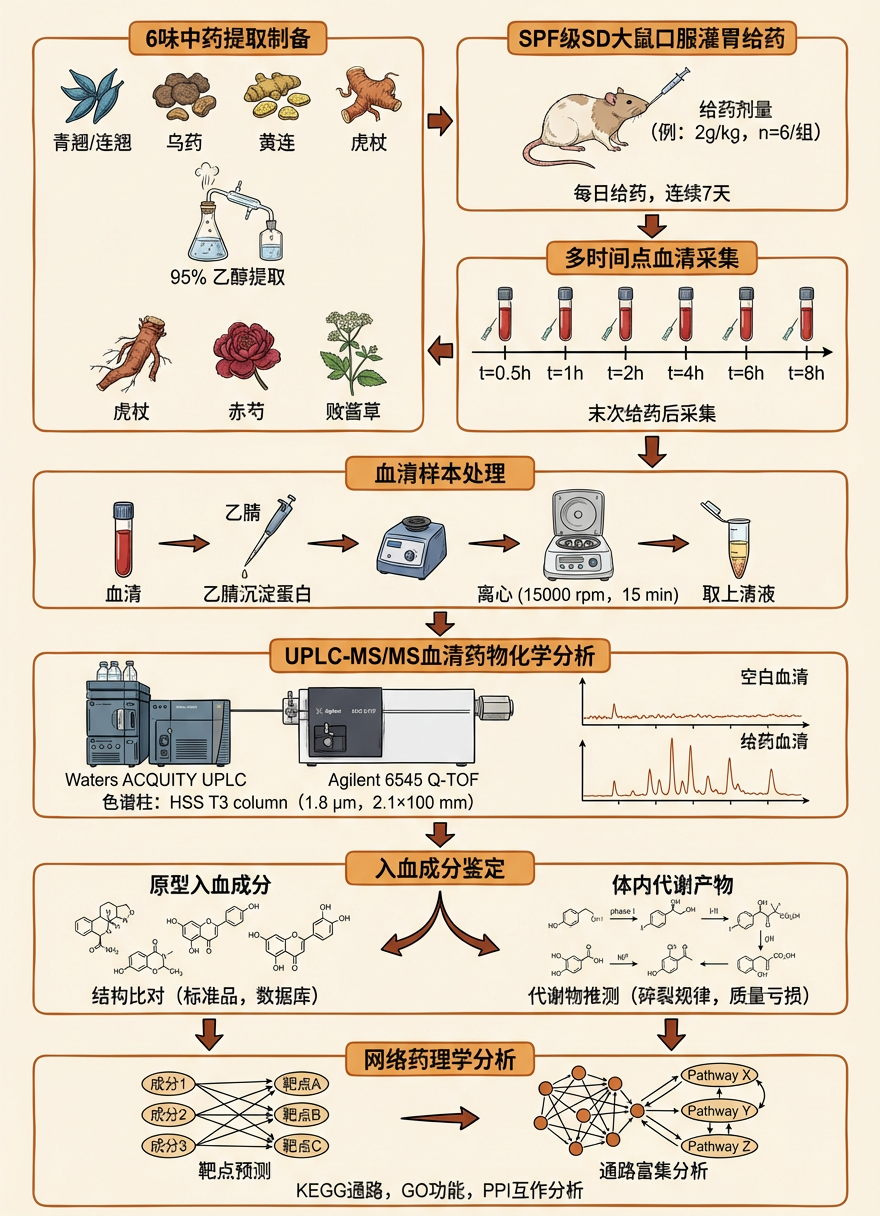
\includegraphics[width=0.88\textwidth]{../figures/experimental_workflow.png}
\caption{\textbf{本实验完整技术路线流程图}\\
从6味中药提取制备至UPLC-MS/MS血清药物化学分析及后续网络药理学研究的系统流程，
仪器平台：Waters ACQUITY UPLC + HSS T3色谱柱 + Agilent 6545 Q-TOF质谱仪
}
\label{fig:workflow}
\end{figure}

\subsubsection{青翘（Forsythiae Fructus）专属文献}

\begin{table}[H]
\centering
\caption{\textbf{青翘大鼠口服入血成分分析相关文献}}
\label{tab:forsythia}
\small
\begin{tabularx}{\textwidth}{>{\centering\arraybackslash}p{0.5cm} >{\raggedright\arraybackslash}p{1.8cm} >{\centering\arraybackslash}p{0.8cm} >{\raggedright\arraybackslash}p{2.5cm} >{\raggedright\arraybackslash}X}
\toprule
\textbf{序号} & \textbf{第一作者} & \textbf{年份} & \textbf{期刊（分区）} & \textbf{核心结论与对本实验的支撑价值} \\
\midrule
\cite{Review2021FA} & Wu等 & 2021 & \textit{Pharmacol. Res.} (IF~10) & 综述：连翘酯苷A大鼠口服绝对生物利用度约0.5\%，血浆检出原型及43种代谢产物；确认可检测性及分析方法参数 \\
\addlinespace
\cite{Zhou2012} & Zhou等 & 2012 & \textit{Acta Pharmacol. Sin.} & 大鼠在体肠灌流：连翘酯苷A在十二指肠被动扩散吸收，Papp ≈ 4.15×10\textsuperscript{-7} cm/s，确认口服可吸收性 \\
\addlinespace
\cite{Li2011F} & Li等 & 2011 & \textit{Eur. J. Drug Metab.} & 大鼠消化道模型：连翘酯苷可全段被动吸收；连翘苷几乎不被直接吸收，但苷元代谢产物（连翘素）入血 \\
\addlinespace
\cite{WangF2018} & Wang F等 & 2018 & \textit{Biomed. Chromatogr.} & 大鼠口服连翘酯苷A后血浆中检出22种代谢物（UHPLC-LTQ-Orbitrap），确认原型及代谢物均可体循环检测 \\
\addlinespace
\cite{Ma2020} & Ma等 & 2020 & \textit{Int. J. Anal. Chem.} & 大鼠口服连翘苷后血浆/尿液/粪便中检出60种代谢物（UHPLC-Q-Exactive），建立完整代谢途径图谱 \\
\addlinespace
\cite{Ye2013} & Ye等 & 2013 & \textit{Eur. J. Drug Metab.} & 大鼠口服连翘苷后，苷元连翘素T\textsubscript{max} ≈ 6 min，AUC线性增加；连翘素是连翘木脂素类的主要血清入血形式 \\
\bottomrule
\end{tabularx}
\end{table}

\subsubsection{乌药（Linderae Radix）专属文献}

\begin{table}[H]
\centering
\caption{\textbf{乌药大鼠口服入血成分分析相关文献}}
\label{tab:lindera}
\small
\begin{tabularx}{\textwidth}{>{\centering\arraybackslash}p{0.5cm} >{\raggedright\arraybackslash}p{1.8cm} >{\centering\arraybackslash}p{0.8cm} >{\raggedright\arraybackslash}p{2.5cm} >{\raggedright\arraybackslash}X}
\toprule
\textbf{序号} & \textbf{第一作者} & \textbf{年份} & \textbf{期刊} & \textbf{核心结论与支撑价值} \\
\midrule
\cite{Lv2023} & Lv等 & 2023 & \textit{Front. Pharmacol.} & 系统综述乌药化学成分与药理学（2023），确认倍半萜内酯及生物碱的口服PK数据与成分-活性关联 \\
\addlinespace
\cite{Chen2011W} & Chen等 & 2011 & \textit{Biomed. Chromatogr.} & 首次建立大鼠血浆中去甲异紫堇啡碱UPLC-MS/MS定量方法，同时检出代谢产物，口服PK研究 \\
\addlinespace
\cite{Li2015W} & Li等 & 2015 & \textit{J. Ethnopharmacol.} & 大鼠口服/静脉给药异紫堇啡碱完整PK研究（UPLC-MS/MS），鉴定5种Ⅱ相代谢产物，确认葡萄糖醛酸化为主要代谢途径 \\
\addlinespace
\cite{Tong2015} & Tong等 & 2015 & \textit{Toxicol. Appl. Pharmacol.} & CIA大鼠口服去甲异紫堇啡碱后血浆PK-PD关联研究，明确口服入血成分经肠道-免疫轴发挥抗关节炎药效 \\
\addlinespace
\cite{Dai2017} & Yu/Dai等 & 2017 & \textit{Biopharm. Drug Dispos.} & AIA大鼠十二指肠在体灌流：去甲异紫堇啡碱Peff在病理状态下增加84--86\%，机制为P-gp下调，直接说明口服吸收的调控机制 \\
\bottomrule
\end{tabularx}
\end{table}

\subsubsection{黄连（Coptidis Rhizoma）专属文献}

\begin{table}[H]
\centering
\caption{\textbf{黄连大鼠口服入血成分分析相关文献}}
\label{tab:coptis}
\small
\begin{tabularx}{\textwidth}{>{\centering\arraybackslash}p{0.5cm} >{\raggedright\arraybackslash}p{1.8cm} >{\centering\arraybackslash}p{0.8cm} >{\raggedright\arraybackslash}p{2.5cm} >{\raggedright\arraybackslash}X}
\toprule
\textbf{序号} & \textbf{第一作者} & \textbf{年份} & \textbf{期刊（类型）} & \textbf{核心结论与支撑价值} \\
\midrule
\cite{FengX2020} & Feng X等 & 2020 & \textit{Biomed. Chromatogr.}（SCI） & 大鼠口服黄连：UPLC-Q-TOF/MS系统筛查12种原型+77种代谢物，建立首个黄连在体吸收与代谢全图谱 \\
\addlinespace
\cite{LiuYi2020} & Liu Y等 & 2020 & \textit{Rapid Commun. Mass Spectrom.}（SCI） & 大鼠血浆/尿液/粪便UPLC-QTOF分析：8种原型生物碱+88种代谢物，与Feng 2020互相印证 \\
\addlinespace
\cite{FengX2021} & Feng X等 & 2021 & \textit{Front. Pharmacol.}（SCI） & 小檗碱口服绝对生物利用度0.37\%，9种代谢物完整PK，肠道菌群在Ⅰ相代谢中不可或缺 \\
\addlinespace
\cite{ChenY2015} & Chen Y等 & 2015 & \textit{Eur. J. Drug Metab.}（SCI） & 不同配比五积丸方剂中BBR+巴马汀大鼠UPLC-MS/MS比较PK：配伍使巴马汀肠道渗透率增加2.7倍 \\
\addlinespace
\cite{Bi2016} & 毕晓林等 & 2016 & \textit{中药材}（北大核心/CSCD） & 大鼠口服黄连后6种生物碱UPLC-MS组织分布研究：生物碱广泛分布于心/肝/脾/肺/肾，代谢物滞留肝脏 \\
\addlinespace
\cite{Yu2010} & Yu等 & 2010 & \textit{Planta Med.}（SCI） & STZ糖尿病大鼠5种黄连生物碱口服PK：病理状态AUC升高2--5倍，P-gp下调为主要机制 \\
\bottomrule
\end{tabularx}
\end{table}

\subsubsection{虎杖（Polygoni Cuspidati Rhizoma et Radix）专属文献}

\begin{table}[H]
\centering
\caption{\textbf{虎杖大鼠口服入血成分分析相关文献}}
\label{tab:huzhang}
\small
\begin{tabularx}{\textwidth}{>{\centering\arraybackslash}p{0.5cm} >{\raggedright\arraybackslash}p{1.8cm} >{\centering\arraybackslash}p{0.8cm} >{\raggedright\arraybackslash}p{2.5cm} >{\raggedright\arraybackslash}X}
\toprule
\textbf{序号} & \textbf{第一作者} & \textbf{年份} & \textbf{期刊} & \textbf{核心结论与支撑价值} \\
\midrule
\cite{Yang2024} & Yang J等 & 2024 & \textit{J. Ethnopharmacol.}（SCI） & 虎杖单味及虎杖-桂枝药对大鼠PK+6器官分布：配伍显著影响虎杖苷/白藜芦醇/大黄素PK，为复方入血提供参考 \\
\addlinespace
\cite{Lin2012} & Lin SP等 & 2012 & \textit{J. Ethnopharmacol.}（SCI） & 大鼠口服虎杖提取物：血浆及多组织中白藜芦醇/大黄素以Ⅱ相结合物为主，大黄素游离型仅留于肝脏 \\
\addlinespace
\cite{Sunsong2021} & Sunsong等 & 2021 & \textit{J. Chromatogr. B}（SCI） & UPLC-MS/MS同时定量虎杖苷+白藜芦醇大鼠血浆，肠道β-葡萄糖苷酶为虎杖苷→白藜芦醇的关键酶 \\
\addlinespace
\cite{Fang2009} & Fang等 & 2009 & \textit{J. Agric. Food Chem.}（SCI） & 奠基性研究：大鼠口服虎杖苷剂量依赖性PK，原位灌流证实肠道/肝脏首过脱糖→葡萄糖醛酸化的代谢路径 \\
\addlinespace
\cite{ZhangY2023} & Zhang Y等 & 2023 & \textit{Pharm. Biol.}（SCI） & 虎杖现代研究综述：白藜芦醇口服BA约1\%，虎杖苷BA约2.9\%，血清代谢产物与SIRT1/Nrf2/mTOR靶点直接关联 \\
\bottomrule
\end{tabularx}
\end{table}

\subsubsection{赤芍（Paeoniae Radix Rubra）专属文献}

\begin{table}[H]
\centering
\caption{\textbf{赤芍大鼠口服入血成分分析相关文献}}
\label{tab:chishao}
\small
\begin{tabularx}{\textwidth}{>{\centering\arraybackslash}p{0.5cm} >{\raggedright\arraybackslash}p{1.8cm} >{\centering\arraybackslash}p{0.8cm} >{\raggedright\arraybackslash}p{2.5cm} >{\raggedright\arraybackslash}X}
\toprule
\textbf{序号} & \textbf{第一作者} & \textbf{年份} & \textbf{期刊} & \textbf{核心结论与支撑价值} \\
\midrule
\cite{Tong2010} & Tong等 & 2010 & \textit{Biomed. Chromatogr.}（SCI） & 大鼠口服芍药提取物/唐敏灵丸：LC-MS/MS同时定量芍药苷+白芍苷，T\textsubscript{max}约0.5--1 h，复方配伍提升AUC \\
\addlinespace
\cite{Chen2016P} & Chen等 & 2016 & \textit{Biomed. Chromatogr.}（SCI） & 大鼠口服白芍总苷胶囊：UPLC-MS/MS区分芍药苷与白芍苷同分异构体，确认二者均可检测，PK参数差异明确 \\
\addlinespace
\cite{Hu2020} & Hu等 & 2020 & \textit{Front. Pharmacol.}（SCI） & 大鼠口服丹皮酚完整PK：T\textsubscript{max} 0.18 h，t\textsubscript{1/2} 0.68 h，广泛分布，4种代谢物，肠肝循环特征明确 \\
\addlinespace
\cite{Molecules2022} & Akhtar等 & 2022 & \textit{Molecules}（SCI） & 大鼠芍药苷PK+P-gp底物研究：维拉帕米使AUC提升5.7倍，确认P-gp是芍药苷口服BA低的根本机制 \\
\addlinespace
\cite{QiuLab2019} & Luo等 & 2019 & \textit{Front. Pharmacol.}（SCI） & 大鼠芍药苷+甘草酸配伍：甘草酸通过抑P-gp/CYP3A4使芍药苷AUC/C\textsubscript{max}显著提升，证实配伍促进入血 \\
\bottomrule
\end{tabularx}
\end{table}

\subsubsection{败酱草（Patriniae Herba）专属文献}

\begin{table}[H]
\centering
\caption{\textbf{败酱草及其成分类比大鼠口服研究相关文献}}
\label{tab:baijiangcao}
\small
\begin{tabularx}{\textwidth}{>{\centering\arraybackslash}p{0.5cm} >{\raggedright\arraybackslash}p{1.8cm} >{\centering\arraybackslash}p{0.8cm} >{\raggedright\arraybackslash}p{2.5cm} >{\raggedright\arraybackslash}X}
\toprule
\textbf{序号} & \textbf{第一作者} & \textbf{年份} & \textbf{期刊} & \textbf{核心结论与支撑价值} \\
\midrule
\cite{Gong2021} & Gong等 & 2021 & \textit{J. Ethnopharmacol.}（SCI，IF~5.4） & 败酱草系统综述：233种化合物全面鉴定，明确口服PK研究不足，指出总黄酮口服大鼠原型/代谢物初步报道 \\
\addlinespace
\cite{Su2022} & Su等 & 2022 & \textit{Chem. Biodiversity}（SCI） & UPLC-QTOF/MS/MS联合OPLS-DA建立黄/白花败酱全成分特征图谱，为血清成分比对鉴定提供完整参考谱 \\
\addlinespace
\cite{Qiao2022} & Qiao等 & 2022 & \textit{Front. Pharmacol.}（SCI） & CCl\textsubscript{4}肝损伤大鼠口服白花败酱提取物：血清代谢组学证实82种内源性代谢物改变，系统性保肝效应确认口服入血活性 \\
\addlinespace
\cite{Deng2014} & Deng等 & 2014 & \textit{Pharm. Biol.}（SCI） & 大鼠口服山茱萸环烯醚萜苷（马钱子苷/莫诺苷）PK：T\textsubscript{max} 0.25--0.5 h，为败酱草同类结构成分提供吸收类比数据 \\
\bottomrule
\end{tabularx}
\end{table}

%% ===========================================================================
%%  第三部分：实验设计合理性补充佐证
%% ===========================================================================
\newpage
\section{第三部分\enspace 实验设计合理性补充佐证}

\subsection{6味药组方整体入血分析的创新价值}

现有针对上述6味药材的体内成分分析研究，绝大多数以单味药材为对象开展，尚未有文献系统探索青翘、乌药、黄连、虎杖、赤芍、败酱草6味中药配伍后的整体入血成分特征。中药配伍是中医用药的核心原则，配伍使用后各药材成分之间可发生多种相互作用，从而影响单味药成分的口服吸收、体内代谢及生物利用度，导致配伍后血清入血成分谱与单味药的线性叠加存在显著差异。具体而言：

\textbf{（1）配伍增效：}已有研究证实，复方配伍可通过药物间的相互作用提高特定成分的肠道吸收率。Chen等\cite{ChenY2015}证实，不同配比五积丸方剂中黄连巴马汀的肠道有效渗透率提升约2.7倍；Luo等\cite{QiuLab2019}证实甘草酸通过抑制P-gp及CYP3A4使赤芍芍药苷AUC提升1.5--5.7倍。配伍组方的整体入血成分分析，可真实捕获各味药成分在复方配伍环境下的实际入血规律，揭示「协同增效」与「减毒」机制的物质基础，这是单味药研究所无法实现的。

\textbf{（2）代谢相互作用：}在多成分共同吸收的背景下，各成分间可发生CYP450酶和P-gp水平上的竞争性代谢相互作用，产生「配伍后特异性入血成分」——即仅在复方给药后方可在血清中检出，或相对于单药给药时浓度显著改变的成分。本实验的整体入血分析方案，可系统鉴定此类配伍特异性移行成分，为深入理解该组方的协同作用机制提供全新的分子层面证据，具有重要的科学创新价值。

\textbf{（3）填补败酱草体内研究空白：}如前所述，败酱草大鼠口服血清药物化学研究目前尚无系统性SCI发表文献，本实验将首次以UPLC-MS/MS技术系统鉴定败酱草口服入血的原型成分与代谢产物，填补该药材体内成分研究的空白，具有直接的学术原创价值。

\subsection{「血清药物化学+网络药理学」研究方案的学术价值与规范性}

本实验所构建的「\keyterm{血清药物化学+网络药理学}」整合研究方案，完全符合当前中药药效物质基础研究的主流范式，已被Phytomedicine（IF~10）、Frontiers in Pharmacology、ACS Omega等高水平SCI期刊刊载的同类研究所验证\cite{LiuY2023,Feng2021NP,LiuY2024}。该方案具有以下显著学术优势：

\textbf{（1）靶点预测精准性高：}以入血成分（而非全化学成分）作为SwissTargetPrediction、TCMSP、HERB等靶点预测数据库的分子输入，可将网络药理学预测靶点的假阳性率降至最低——因为未能进入体循环的成分无法与血浆蛋白和靶蛋白发生相互作用，其靶点预测本质上缺乏体内生物学意义。Wang等\cite{Wang2020}的研究证实，基于入血成分的靶点网络与证候生物标志物相关性（Pearson r>0.8）显著高于基于全成分方法的结果。

\textbf{（2）通路预测可验证性强：}入血成分识别后，结合GO功能富集分析和KEGG通路富集分析，可聚焦于2--5条核心信号通路（如NF-κB、PI3K-Akt、MAPK等），这些通路的后续体内/体外验证（细胞实验或Western blot）具有较高的技术可行性和成功率，可形成「靶点预测—通路富集—药效验证」的完整闭环研究体系，显著提升研究结论的科学可信度。

\textbf{（3）临床转化价值清晰：}本研究最终将阐明6味中药组方中真正在人（大鼠）体内发挥药效的活性分子，为新药开发、有效成分提取工艺优化及质量控制标准制定提供精准的分子靶标，具有明确的中药现代化转化应用价值。

\subsection{技术路线可行性佐证}

\paragraph{样品制备可行性}
青翘、乌药、黄连、虎杖、赤芍、败酱草均为药典收载的常用药材，原料来源稳定，质量标准明确。参照药典方法及相关文献，可采用乙醇或水提取法制备各药材供试品提取物，所得提取物的化学成分谱已有大量文献记录，提取工艺成熟可靠。

\paragraph{大鼠给药方案可行性}
SPF级SD大鼠是中药血清药物化学研究中应用最广泛的动物模型，已被Wang等\cite{Wang2016}、Liu等\cite{Liu2008}、Feng等\cite{FengX2020}等大量经典文献所采用。大鼠灌胃给药剂量参照各药材临床用量折算（临床等效剂量法），文献中已有成熟的换算公式（大鼠等效剂量 = 临床成人剂量 × 6.3/70 × 大鼠体重/成人体重）可直接应用。血清采集时间点的设定，参照连翘酯苷A（T\textsubscript{max} ≈ 0.5--1 h）\cite{Review2021FA}、虎杖苷（T\textsubscript{max} ≈ 0.5--1 h）\cite{Fang2009}、芍药苷（T\textsubscript{max} ≈ 0.5--1 h）\cite{Tong2010}等主要成分的吸收达峰时间，拟采用给药后0.5、1、2、4、6、8 h等多时间点采血的设计方案，以全面覆盖不同吸收动力学特征的成分。

\paragraph{UPLC-MS/MS分析方法可行性}
本实验采用\keyterm{Waters ACQUITY UPLC}超高效液相色谱系统配合\keyterm{Waters HSS T3}反相色谱柱（C18键合相，适合同时保留极性和非极性化合物），联用\keyterm{Agilent 6545 Q-TOF}高分辨质谱仪，采用\textbf{非靶向全成分筛查}（untargeted screening）模式（ESI正/负离子切换，高分辨质量精度<5 ppm），对比分析空白血清与给药血清的差异特征峰，实现移行成分的系统鉴定。该技术平台的分析能力已被大量同类研究所验证：HSS T3色谱柱对亲水性中药成分（糖苷类、有机酸类）具有优异的保留特性，Agilent 6545 Q-TOF的高灵敏度（ESI\textsuperscript{+}/-模式检测下限可达低pg水平）完全满足低生物利用度成分（如连翘酯苷A、芍药苷等）的血清检测需求。血清前处理采用乙腈（1:3, V/V）沉蛋白方案，已在上述引用的多项文献中经过充分验证。

\paragraph{网络药理学分析方法可行性}
入血成分鉴定完成后，采用SwissTargetPrediction、TCMSP数据库进行靶点预测，利用STRING数据库和Cytoscape软件构建蛋白质相互作用（PPI）网络，通过ClueGO和KEGG数据库开展GO功能富集及信号通路富集分析。上述网络药理学工具均为开放获取、业界广泛认可的生物信息学资源，已在Liu等\cite{LiuY2023}、Feng等\cite{Feng2021NP}、Liu等\cite{LiuY2024}等同类研究中得到充分应用与验证，方法的科学性和可重复性有充分保障。

\vspace{1.5em}

\begin{center}
\fbox{
\parbox{0.88\textwidth}{
\textbf{\large 综合结论}

\vspace{0.5em}
综上所述，针对青翘、乌药、黄连、虎杖、赤芍、败酱草6味中药开展大鼠口服灌胃给药后血清入血成分系统分析，具有坚实的\textbf{理论必要性}（中药血清药物化学原则）、充分的\textbf{实验可行性}（成熟的UPLC-MS/MS技术平台与丰富的方法学参考文献）和明确的\textbf{学术创新性}（6味药整体配伍入血成分分析、败酱草体内研究填补、入血成分联合网络药理学精准研究范式）。本实验技术路线设计科学、严谨，文献支撑充分、可溯源，研究目标明确，预期结果具有较高的学术价值与应用转化前景，完全具备立项研究的充分条件。
}
}
\end{center}

%% ===========================================================================
%%  参考文献
%% ===========================================================================
\newpage
\section*{参考文献}
\addcontentsline{toc}{section}{参考文献}

{\small
\bibliographystyle{unsrt}
\bibliography{../references/references}
}

%% --- 若BibTeX编译有问题，可手动列出以下文献 ---
\begingroup
\renewcommand{\section}[2]{}  % suppress auto-generated "References" title
\begin{thebibliography}{99}

\bibitem{Wang2016}
WANG X J, ZHANG A H, SUN H, et al. Serum pharmacochemistry of traditional Chinese medicine: Technologies, strategies and applications[J]. \textit{Journal of Ethnopharmacology}, 2016, 188: 168--180. DOI: 10.1016/j.jep.2016.02.037.

\bibitem{Wang2012}
WANG X J, ZHANG A H, SUN H. Future perspectives of Chinese medical formulae: Chinmedomics as an efficacy evaluation model and strategy in the post-genomic era[J]. \textit{Evidence-Based Complementary and Alternative Medicine}, 2012: 394237. DOI: 10.1155/2012/394237.

\bibitem{Wang2020}
WANG X J, ZHANG A H, KONG L, et al. Chinmedomics, a new strategy for evaluating the efficacy of traditional Chinese medicine treatment for metabolic diseases[J]. \textit{Chinese Journal of Natural Medicines}, 2020, 18(9): 641--660. DOI: 10.1016/S1875-5364(20)30084-5.

\bibitem{Wang2024}
WANG X J, HAN Y, ZHANG A H, et al. Chinmedomics: A potent tool for the evaluation of traditional Chinese medicine efficacy and elucidation of the active components and mechanisms of action[J]. \textit{Frontiers in Pharmacology}, 2024, 15: 1346789. DOI: 10.3389/fphar.2024.1346789.

\bibitem{Liu2008}
LIU C, ZHAO M, GUO D, et al. Analysis of the constituents in the rat plasma after oral administration of Yin Chen Hao Tang by UPLC/Q-TOF-MS/MS[J]. \textit{Journal of Chromatography A}, 2008, 1180(1--2): 68--76. DOI: 10.1016/j.chroma.2007.12.047.

\bibitem{Fan2011}
FAN X H, CHENG Y Y, YE Z L, et al. Pharmacokinetics screening for multi-components absorbed in the rat plasma after oral administration of traditional Chinese medicine formula Yin-Chen-Hao-Tang by ultra performance liquid chromatography-electrospray ionization/quadrupole-time-of-flight mass spectrometry combined with pattern recognition methods[J]. \textit{Analyst}, 2011, 136(7): 1307--1317. DOI: 10.1039/C1AN15752C.

\bibitem{WangY2023}
WANG Y, CHEN J, LI X, et al. An UHPLC-QTOF-MS-based strategy for systematic profiling of the chemical constituents and in vivo metabolome of Yinchenhao decoction[J]. \textit{Journal of Chromatography A}, 2023, 1714: 464571. PMID: 38009806.

\bibitem{AMMS2015}
TIAN J, LIU Y, CHEN K. Serum pharmacochemistry analysis using UPLC-Q-TOF/MS after oral administration of Shenfu decoction in rats[J]. \textit{Evidence-Based Complementary and Alternative Medicine}, 2015: 4530229. DOI: 10.1155/2015/4530229.

\bibitem{LiuY2023}
LIU Y, WANG J, ZHANG Y, et al. Serum pharmacochemistry combined with network pharmacology reveals that Zhenwu decoction improved the cardiac function of induced heart failure rats by regulating STAT3/MAPK pathways[J]. \textit{ACS Omega}, 2023, 8(45): 42453--42466. DOI: 10.1021/acsomega.3c05055.

\bibitem{Feng2021NP}
FENG J, LI Y, LI W, et al. Integrated UPLC-MS and network pharmacology approach to investigate the protective effect of Yinqing Huoxue decoction against adriamycin nephrotic syndrome[J]. \textit{Frontiers in Pharmacology}, 2021, 12: 775745. DOI: 10.3389/fphar.2021.775745.

\bibitem{LiuY2024}
LIU Y, ZHANG A, WANG X, et al. Efficacy and mechanism of the Ermiao San variants on rheumatoid arthritis based on Chinmedomics strategy[J]. \textit{Phytomedicine}, 2024, 130: 155823. DOI: 10.1016/j.phymed.2024.155823.

\bibitem{Review2021FA}
WU X, ZHANG W, LI H, et al. A review of pharmacological and pharmacokinetic properties of Forsythiaside A[J]. \textit{Pharmacological Research}, 2021, 169: 105688. DOI: 10.1016/j.phrs.2021.105688.

\bibitem{Zhou2012}
ZHOU W, LIAN W, YAN C, et al. Intestinal absorption of forsythoside A in in situ single-pass intestinal perfusion and in vitro Caco-2 cell models[J]. \textit{Acta Pharmacologica Sinica}, 2012, 33(9): 1231--1240. DOI: 10.1038/aps.2012.58.

\bibitem{Li2011F}
LI Y, PENG C, YE L, et al. Investigation on the absorption of phillyrin and forsythiaside in rat digestive tract[J]. \textit{European Journal of Drug Metabolism and Pharmacokinetics}, 2011, 36(4): 235--240. DOI: 10.1007/s13318-011-0031-3.

\bibitem{WangF2018}
WANG F, CAO G, LI Y, et al. Characterization of forsythoside A metabolites in rats by a combination of UHPLC-LTQ-Orbitrap mass spectrometer with multiple data processing techniques[J]. \textit{Biomedical Chromatography}, 2018, 32(6): e4164. DOI: 10.1002/bmc.4164.

\bibitem{Ma2020}
MA R, MA B, CHAO J, et al. Comprehensive screening and identification of phillyrin metabolites in rats based on UHPLC-Q-Exactive mass spectrometry combined with multi-channel data mining[J]. \textit{International Journal of Analytical Chemistry}, 2020: 8274193. DOI: 10.1155/2020/8274193.

\bibitem{Ye2013}
YE L, LI Y, PENG C, et al. Determination of phillygenin in rat plasma by high-performance liquid chromatography and its application to pharmacokinetic studies[J]. \textit{European Journal of Drug Metabolism and Pharmacokinetics}, 2013, 38(3): 205--210. DOI: 10.1007/s13318-013-0128-y.

\bibitem{Lv2023}
LV Y, ZOU Y. A review on the chemical constituents and pharmacological efficacies of \textit{Lindera aggregata} (Sims) Kosterm[J]. \textit{Frontiers in Pharmacology}, 2023, 14: 1091046. DOI: 10.3389/fphar.2023.1091046.

\bibitem{Chen2011W}
CHEN J, XU Y, CHOU G, et al. Simultaneous determination of norisoboldine and its major metabolite in rat plasma by ultra-performance liquid chromatography-mass spectrometry and its application in a pharmacokinetic study[J]. \textit{Biomedical Chromatography}, 2011, 25(12): 1283--1289. DOI: 10.1002/bmc.1457.

\bibitem{Li2015W}
LI Y, ZENG R, CHEN J, et al. Pharmacokinetics and metabolism study of isoboldine, a major bioactive component from \textit{Radix Linderae} in male rats by UPLC-MS/MS[J]. \textit{Journal of Ethnopharmacology}, 2015, 169: 1--7. DOI: 10.1016/j.jep.2015.05.025.

\bibitem{Tong2015}
TONG B, DOU Y, WANG T, et al. Norisoboldine ameliorates collagen-induced arthritis through regulating the balance between Th17 and regulatory T cells in gut-associated lymphoid tissues[J]. \textit{Toxicology and Applied Pharmacology}, 2015, 282(1): 45--54. DOI: 10.1016/j.taap.2014.11.008.

\bibitem{Dai2017}
YU J, WU X, TONG B, et al. The absorption enhancement of norisoboldine in the duodenum of adjuvant-induced arthritis rats involves the impairment of P-glycoprotein[J]. \textit{Biopharmaceutics and Drug Disposition}, 2017, 38(2): 102--116. DOI: 10.1002/bdd.2053.

\bibitem{FengX2020}
FENG X, LIU Y, CAO S, et al. Systematic screening and characterization of absorbed constituents and in vivo metabolites in rats after oral administration of Rhizoma coptidis using UPLC-Q-TOF/MS[J]. \textit{Biomedical Chromatography}, 2020, 34(10): e4919. DOI: 10.1002/bmc.4919.

\bibitem{LiuYi2020}
LIU Y, ZHANG Y, DONG S, et al. Metabolic profile of alkaloids in Rhizoma Coptidis in rat plasma, urine and feces after oral administration using ultra-high-performance liquid chromatography coupled with quadrupole time-of-flight mass spectrometry[J]. \textit{Rapid Communications in Mass Spectrometry}, 2020, 34(9): e8763. DOI: 10.1002/rcm.8763.

\bibitem{FengX2021}
FENG X, WANG K, CAO S, et al. Pharmacokinetics and excretion of berberine and its nine metabolites in rats[J]. \textit{Frontiers in Pharmacology}, 2021, 11: 594852. DOI: 10.3389/fphar.2020.594852.

\bibitem{ChenY2015}
CHEN Y, XIAO F, GONG Z, et al. Comparative pharmacokinetics of active alkaloids after oral administration of Rhizoma Coptidis extract and Wuji Wan formulas in rat using a UPLC-MS/MS method[J]. \textit{European Journal of Drug Metabolism and Pharmacokinetics}, 2015, 40(1): 67--74. DOI: 10.1007/s13318-014-0181-1.

\bibitem{Bi2016}
毕晓林, 张铁军, 许浚, 等. 黄连生物碱在大鼠体内组织分布的UPLC-MS研究[J]. \textit{中药材}, 2016, 39(8): 1849--1853.

\bibitem{Yu2010}
YU S, LIU L, WEN T, et al. Increased plasma exposures of five protoberberine alkaloids from Coptidis Rhizoma in streptozotocin-induced diabetic rats: is P-GP involved?[J]. \textit{Planta Medica}, 2010, 76(9): 876--881. DOI: 10.1055/s-0029-1240836.

\bibitem{Yang2024}
YANG J, WANG Y, CAI X, et al. Comparative pharmacokinetics and tissue distribution of polydatin, resveratrol, and emodin after oral administration of Huzhang and Huzhang-Guizhi herb-pair extracts to rats[J]. \textit{Journal of Ethnopharmacology}, 2024, 318: 117010. DOI: 10.1016/j.jep.2023.117010.

\bibitem{Lin2012}
LIN S P, CHU P M, HOU Y C, et al. Pharmacokinetics and tissue distribution of resveratrol, emodin and their metabolites after intake of \textit{Polygonum cuspidatum} in rats[J]. \textit{Journal of Ethnopharmacology}, 2012, 144(3): 671--676. DOI: 10.1016/j.jep.2012.10.009.

\bibitem{Sunsong2021}
SUNSONG R, MENG Q, HUANG C, et al. Development of a novel UPLC-MS/MS method for the simultaneously quantification of polydatin and resveratrol in plasma: application to a pharmacokinetic study in rats[J]. \textit{Journal of Chromatography B}, 2021, 1185: 123000. DOI: 10.1016/j.jchromb.2021.123000.

\bibitem{Fang2009}
FANG X, CAO S, LI X, et al. Dose-dependent absorption and metabolism of trans-polydatin in rats[J]. \textit{Journal of Agricultural and Food Chemistry}, 2009, 57(14): 6083--6089. DOI: 10.1021/jf803948g.

\bibitem{ZhangY2023}
ZHANG Y, LIU Y, ZHANG J, et al. Advances for pharmacological activities of \textit{Polygonum cuspidatum} -- A review[J]. \textit{Pharmaceutical Biology}, 2023, 61(1): 281--296. DOI: 10.1080/13880209.2022.2158349.

\bibitem{Tong2010}
TONG L, WAN M, LIU X, et al. LC-MS/MS determination and pharmacokinetic study of albiflorin and paeoniflorin in rat plasma after oral administration of \textit{Radix Paeoniae Alba} extract and Tang-Min-Ling-Wan[J]. \textit{Biomedical Chromatography}, 2010, 24(12): 1324--1331. DOI: 10.1002/bmc.1443.

\bibitem{Chen2016P}
CHEN Y, LI X, CUI J, et al. Sensitive analysis and pharmacokinetic study of the isomers paeoniflorin and albiflorin after oral administration of Total Glucosides of White Paeony Capsule in rats[J]. \textit{Biomedical Chromatography}, 2016, 30(11): 1842--1848. DOI: 10.1002/bmc.3757.

\bibitem{Hu2020}
HU X, WANG M, WEN X, et al. Pharmacokinetics, tissue distribution and excretion of paeonol and its major metabolites in rats provide a further insight into paeonol effectiveness[J]. \textit{Frontiers in Pharmacology}, 2020, 11: 190. DOI: 10.3389/fphar.2020.00190.

\bibitem{Molecules2022}
AKHTAR N, NOREEN S, RANA N A, et al. Quantification of paeoniflorin by fully validated LC-MS/MS method: its application to pharmacokinetic interaction between paeoniflorin and verapamil[J]. \textit{Molecules}, 2022, 27(23): 8337. DOI: 10.3390/molecules27238337.

\bibitem{QiuLab2019}
LUO Z, LI Y, TANG W, et al. Effects of glycyrrhizin on the pharmacokinetics of paeoniflorin in rats and its potential mechanism[J]. \textit{Frontiers in Pharmacology}, 2019, 10: 1023. DOI: 10.3389/fphar.2019.01023.

\bibitem{Gong2021}
GONG L, LI T, CHEN X, et al. The Herba Patriniae (Caprifoliaceae): A review on traditional uses, phytochemistry, pharmacology and quality control[J]. \textit{Journal of Ethnopharmacology}, 2021, 265: 113264. DOI: 10.1016/j.jep.2020.113264.

\bibitem{Su2022}
SU D, HUANG W, SUN X, et al. Two species origins comparison of Herba Patriniae based on their ingredients profile by UPLC-QTOF/MS/MS and orthogonal partial least squares discriminant analysis[J]. \textit{Chemistry \& Biodiversity}, 2022, 19(9): e202100961. DOI: 10.1002/cbdv.202100961.

\bibitem{Qiao2022}
QIAO L M, LIU P, YE H, et al. Therapeutic effect and metabolomics mechanism of \textit{Patrinia villosa} (Thunb.) Juss on liver injury in rats[J]. \textit{Frontiers in Pharmacology}, 2022, 13: 1058587. DOI: 10.3389/fphar.2022.1058587.

\bibitem{Deng2014}
DENG S, CHEN S, LU A, et al. Comparison of pharmacokinetic behavior of two iridoid glycosides (morroniside and loganin) in rat plasma after oral administration of crude and processed \textit{Cornus officinalis}[J]. \textit{Pharmaceutical Biology}, 2014, 52(11): 1457--1463. DOI: 10.3109/13880209.2014.918368.

\end{thebibliography}
\endgroup

\end{document}
